\subsection{Finalizing the datapath}
\begin{figure}[ht]
    \centering
    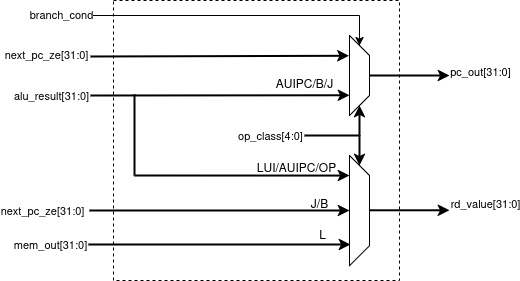
\includegraphics[scale = 0.45]{WB_BD.png}
    \caption{Write Back block diagram}
    \label{fig:WB_BD}
\end{figure}

The final pieces that remain to be designed are the one that manages the Data Memory, and decides when to write, and the stage which, depending on the operation type, selects what to return as new value for the PC and what to store in the destination register, i.e the Write Back.\\
The Data Memory will instantiated as a 16KB single port RAM and separated from the rest, forming a 5-stage datapath when it is going to be pipelined. In 4-stages architecture it would be instead included in the same block, reducing the overall size of the processor, reducing power consumption, due to the presence of one less register, but at the cost of a reduced throughput. 

\subsection{Simulating an unpipelined datapath}